\documentclass[11pt,a4paper]{article}

\usepackage[margin=1in]{geometry}
\usepackage{titlesec}
\usepackage{enumitem}
\usepackage{hyperref}
\usepackage{parskip}
\usepackage{graphicx}
\usepackage{float}
\usepackage{xcolor}
\usepackage{listings}
\usepackage{booktabs}
\usepackage{ragged2e}

\hypersetup{
    colorlinks=true,
    linkcolor=blue,
    urlcolor=blue
}

\titleformat{\section}{\large\bfseries}{\thesection}{0.5em}{}
\titleformat{\subsection}{\normalsize\bfseries}{\thesubsection}{0.5em}{}

% Code listing style
\definecolor{codebg}{rgb}{0.96,0.96,0.96}
\definecolor{codekw}{rgb}{0.13,0.29,0.53}
\definecolor{codecomment}{rgb}{0.30,0.55,0.30}
\definecolor{codestr}{rgb}{0.64,0.08,0.08}

\lstdefinestyle{py}{
    language=Python,
    backgroundcolor=\color{codebg},
    basicstyle=\ttfamily\small,
    keywordstyle=\color{codekw}\bfseries,
    commentstyle=\color{codecomment}\itshape,
    stringstyle=\color{codestr},
    numbers=left,
    numberstyle=\tiny\color{gray},
    numbersep=8pt,
    showstringspaces=false,
    breaklines=true,
    frame=single,
    rulecolor=\color{gray!40},
    tabsize=4,
    captionpos=b
}

\lstdefinestyle{sql}{
    language=SQL,
    backgroundcolor=\color{codebg},
    basicstyle=\ttfamily\small,
    keywordstyle=\color{codekw}\bfseries,
    stringstyle=\color{codestr},
    showstringspaces=false,
    breaklines=true,
    frame=single,
    rulecolor=\color{gray!40},
    captionpos=b
}

\title{\vspace{-1.5cm}\textbf{PKCERT AI \& Software Development Internship \\ Task 05: Data Preprocessing, Visualization \& SQL}}
\author{Abdullah Amir}
\date{AI and Software Development \\ 08 July 2026}

\begin{document}

\maketitle
\vspace{-1cm}

\tableofcontents
\vspace{0.5cm}

% ======================================================================
\section*{Overview}
\addcontentsline{toc}{section}{Overview}
For this task I worked with the \textbf{New York City Airbnb Open Data (2019)} from Kaggle. It lists close to 49,000 Airbnb listings across the five boroughs, with a nice mix of numeric columns (price, minimum nights, number of reviews) and categorical ones (borough, neighbourhood, room type). It also has genuine missing values and some wild outliers, which makes it a realistic dataset to clean rather than a tidy toy example.

Everything below is produced by a single script, \texttt{airbnb\_analysis.py}, which runs in four stages: it cleans the raw CSV, draws five figures, builds encoded and scaled feature tables, and finally loads the clean data into a small SQLite database and queries it from Python. The dataset has 16 columns and 48,895 rows to start with.

% ======================================================================
\section*{Part A: Data Cleaning and Preprocessing}
\addcontentsline{toc}{section}{Part A: Data Cleaning and Preprocessing}

\subsection*{Missing Values}
The first thing I checked was where the gaps were. Four columns had missing values: \texttt{name} (16), \texttt{host\_name} (21), and both \texttt{last\_review} and \texttt{reviews\_per\_month} (10,052 each). The two review columns are missing together, and that is the clue to what is going on: those listings have simply never been reviewed.

\begin{lstlisting}[style=py, caption={Handling the missing values column by column.}]
# name / host_name: only a handful missing, fill with a placeholder
df["name"] = df["name"].fillna("Unknown")
df["host_name"] = df["host_name"].fillna("Unknown")

# reviews_per_month: missing means the listing was never reviewed,
# so the right value is 0, not the mean or median
df["reviews_per_month"] = df["reviews_per_month"].fillna(0)

# last_review: a date that only exists for reviewed listings.
# We do not use it in the numeric analysis, so we drop the column.
df = df.drop(columns=["last_review"])
\end{lstlisting}

The reasoning behind each choice: \texttt{name} and \texttt{host\_name} are just text labels with a few gaps, so a plain ``Unknown'' placeholder keeps the rows without pretending we know something. For \texttt{reviews\_per\_month} the missing value genuinely means zero reviews per month, so filling with 0 is the honest answer. \texttt{last\_review} is a date that only makes sense for listings that were reviewed, and since it plays no part in the numeric work, I dropped the whole column rather than invent dates.

\subsection*{Duplicate Records}
Next I looked for duplicates, both fully repeated rows and repeated listing ids (since \texttt{id} should be unique per listing).

\begin{lstlisting}[style=py, caption={Checking for duplicates.}]
print(df.duplicated().sum())            # fully duplicated rows -> 0
print(df.duplicated(subset="id").sum()) # duplicated ids       -> 0
df = df.drop_duplicates()
df = df.drop_duplicates(subset="id")
\end{lstlisting}

This dataset turned out to be clean on that front: zero fully duplicated rows and zero repeated ids. I still ran the drop calls so the pipeline stays safe if the data is ever refreshed with duplicates in it.

\subsection*{Outliers}
Price and minimum nights both had unrealistic extremes. Eleven listings had a price of 0, which cannot be a real nightly rate, so those went first. For the rest of the price column I used the classic IQR rule: anything above the upper fence (Q3 plus 1.5 times the interquartile range) is treated as an outlier.

\begin{lstlisting}[style=py, caption={Removing outliers from price and minimum nights.}]
# price = 0 is not a valid nightly rate
df = df[df["price"] > 0]

# IQR rule on price to trim the extreme right tail
q1, q3 = df["price"].quantile([0.25, 0.75])
upper_fence = q3 + 1.5 * (q3 - q1)      # about 334
df = df[df["price"] <= upper_fence]

# a minimum stay over a year is unrealistic for a short-term rental
df = df[df["minimum_nights"] <= 365]
\end{lstlisting}

The price fence came out at about \$334. That flagged 2,972 listings on the high end, which I removed to stop a handful of luxury outliers from dominating every chart and average. I also dropped 13 listings that asked for a minimum stay of more than a year, since those are clearly not normal short-term rentals. After all of this the dataset went from 48,895 rows down to a clean \textbf{45,899 rows}, which I saved to \texttt{airbnb\_cleaned.csv}.

% ======================================================================
\section*{Part B: Data Visualization}
\addcontentsline{toc}{section}{Part B: Data Visualization}
With clean data in hand I drew five figures using Matplotlib and Seaborn. Each one is saved into the \texttt{figures/} folder by the script.

\subsection*{1. Histogram: Price Distribution}
\begin{figure}[H]
    \centering
    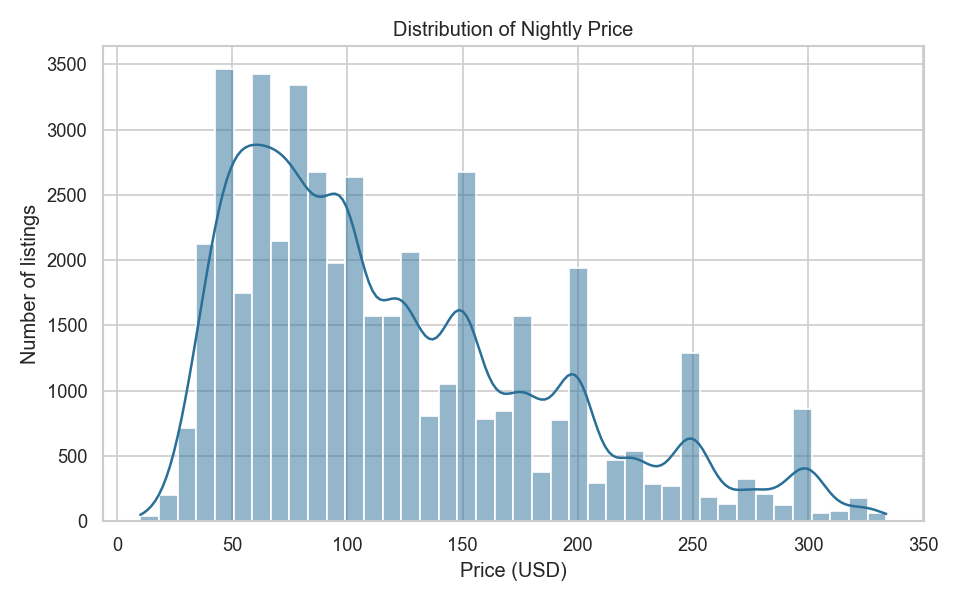
\includegraphics[width=0.8\textwidth]{figures/01_histogram_price.png}
    \caption{Distribution of nightly price after cleaning.}
\end{figure}
The price distribution is strongly right skewed. Most listings sit between roughly \$50 and \$150 a night, and the count tails off steadily after that. The little spikes at round numbers like 100, 150, and 200 are a nice human detail: hosts clearly love pricing at round figures rather than something like \$147.

\subsection*{2. Boxplot: Price by Room Type}
\begin{figure}[H]
    \centering
    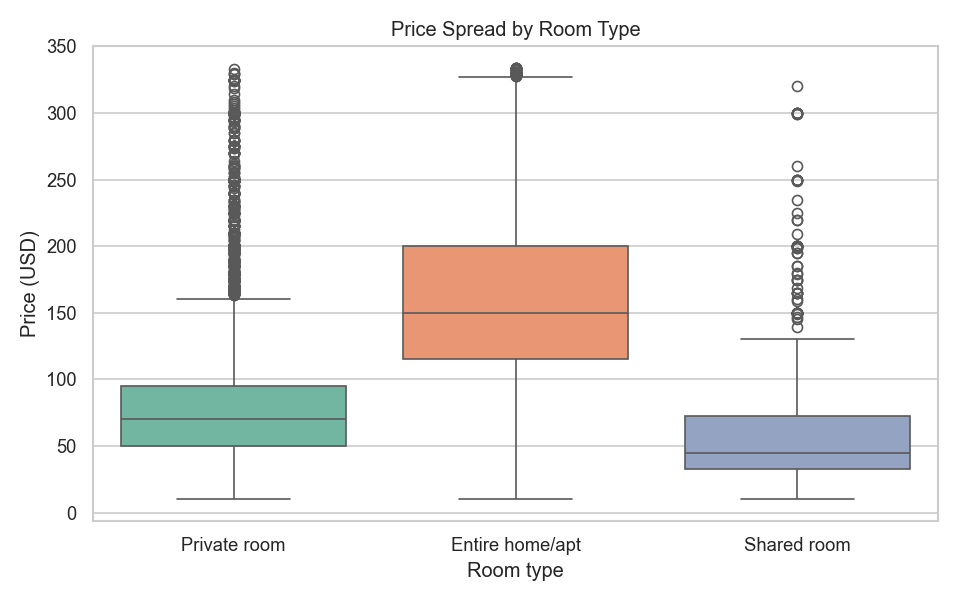
\includegraphics[width=0.8\textwidth]{figures/02_boxplot_price_roomtype.png}
    \caption{Price spread for each room type.}
\end{figure}
Splitting price by room type shows exactly the ordering you would expect. An entire home or apartment has the highest median (around \$150) and the widest spread, a private room sits lower (around \$70), and a shared room is cheapest of all. Even after trimming outliers there are still dots above the whiskers, which just means each room type has its own pricier listings relative to its group.

\subsection*{3. Correlation Heatmap}
\begin{figure}[H]
    \centering
    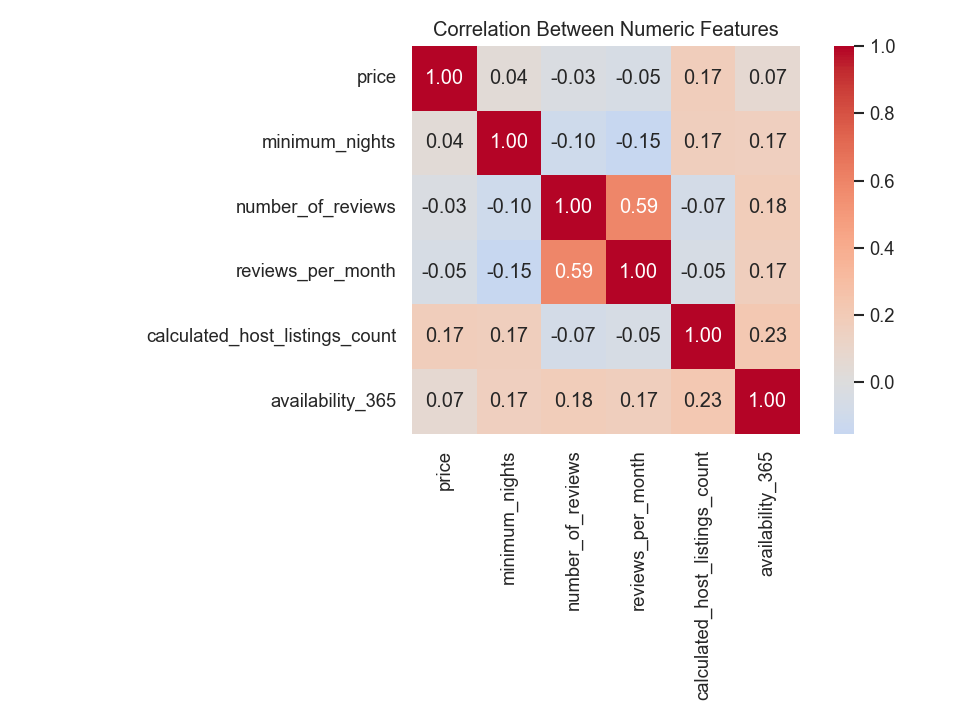
\includegraphics[width=0.72\textwidth]{figures/03_correlation_heatmap.png}
    \caption{Correlation between the numeric features.}
\end{figure}
The heatmap looks for linear relationships between the numeric columns. The strongest one is between \texttt{number\_of\_reviews} and \texttt{reviews\_per\_month} at 0.59, which makes sense as both measure review activity. What stands out just as much is what is \emph{not} there: price barely correlates with anything numeric (all close to 0), which tells me that price is driven mostly by the categorical features like room type and borough rather than by counts of reviews or availability.

\subsection*{4. Average Price by Borough}
\begin{figure}[H]
    \centering
    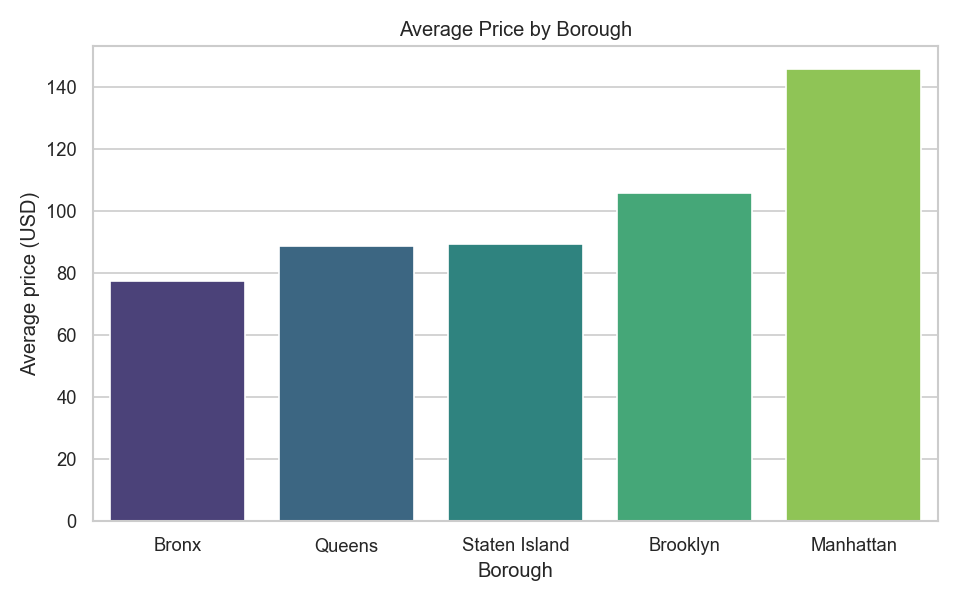
\includegraphics[width=0.8\textwidth]{figures/04_avgprice_by_borough.png}
    \caption{Average nightly price in each borough.}
\end{figure}
This bar chart confirms the point the heatmap hinted at. Manhattan is comfortably the most expensive borough on average (around \$146), Brooklyn follows (around \$106), and the Bronx is the cheapest (around \$77). Location carries a lot of the price signal.

\subsection*{5. Listings Map by Borough}
\begin{figure}[H]
    \centering
    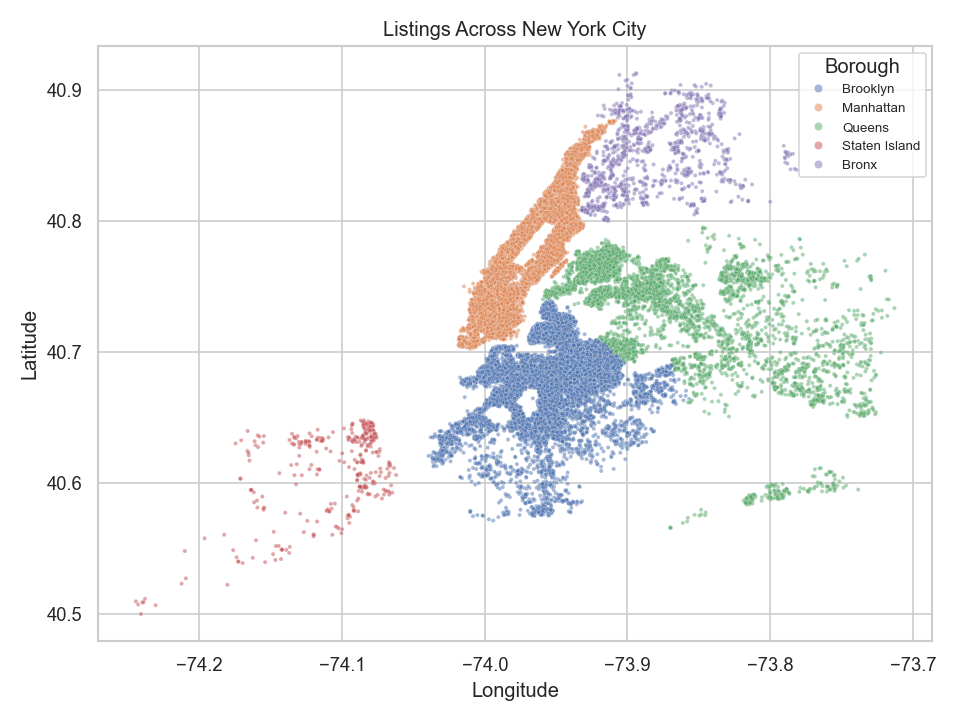
\includegraphics[width=0.8\textwidth]{figures/05_scatter_map.png}
    \caption{Every listing plotted by longitude and latitude, coloured by borough.}
\end{figure}
Plotting each listing by its longitude and latitude basically redraws the map of New York City without ever loading a map. The colours separate cleanly into the five boroughs, and you can see how densely packed Manhattan and Brooklyn are compared with the sparse scatter of Staten Island. It is a good reminder that latitude and longitude are real features, not just ID numbers.

% ======================================================================
\section*{Part C: Feature Engineering}
\addcontentsline{toc}{section}{Part C: Feature Engineering}
Before any machine learning model can use this data, the text columns need to become numbers and the numeric columns need to be on a comparable scale.

\subsection*{Identifying and Encoding Categorical Features}
The categorical columns are \texttt{name}, \texttt{host\_name}, \texttt{neighbourhood\_group}, \texttt{neighbourhood}, and \texttt{room\_type}. The two that matter for modelling are the low-cardinality \texttt{neighbourhood\_group} (5 values) and \texttt{room\_type} (3 values), plus \texttt{neighbourhood} which has 219 distinct values.

\begin{lstlisting}[style=py, caption={Label encoding and one-hot encoding.}]
from sklearn.preprocessing import LabelEncoder

# Label Encoding: one integer code per category.
# Good for a high-cardinality column like neighbourhood (219 values).
le = LabelEncoder()
fe["neighbourhood_encoded"] = le.fit_transform(fe["neighbourhood"])

# One-Hot Encoding: one 0/1 column per category.
# Good for low-cardinality columns, avoids a fake ordering.
fe = pd.get_dummies(fe,
        columns=["neighbourhood_group", "room_type"],
        prefix=["borough", "room"])
\end{lstlisting}

I used the two encoders deliberately for different jobs. \textbf{Label encoding} turns each category into a single integer, which is compact and works well for \texttt{neighbourhood} where 219 one-hot columns would be wasteful. The catch is that it invents an ordering (code 5 looks ``bigger'' than code 2 even when the categories are not ranked). \textbf{One-hot encoding} avoids that by giving each category its own 0/1 column, so no false ordering sneaks in. That is why I used it for \texttt{neighbourhood\_group} and \texttt{room\_type}, which produced columns like \texttt{borough\_Manhattan} and \texttt{room\_Private room}.

\subsection*{Normalization and Standardization}
The numeric columns live on very different scales: price runs into the hundreds while \texttt{reviews\_per\_month} is usually near 1. If you feed those straight into a distance-based or gradient-based model, the large-valued columns drown out the small ones. Standardization fixes this by rescaling each column to a mean of 0 and a standard deviation of 1.

\begin{lstlisting}[style=py, caption={Standardizing the numeric features.}]
from sklearn.preprocessing import StandardScaler

num_cols = ["price", "minimum_nights", "number_of_reviews",
            "reviews_per_month", "calculated_host_listings_count",
            "availability_365"]
scaler = StandardScaler()
scaled = scaler.fit_transform(df[num_cols])
# every scaled column now has mean ~0 and std ~1
\end{lstlisting}

After scaling, every one of those columns has a mean of essentially 0 and a standard deviation of 1, so they all contribute on equal footing. This matters for models like k-nearest neighbours, SVMs, and anything using gradient descent, where features on a huge scale would otherwise dominate the result purely because of their units. The engineered table is saved to \texttt{airbnb\_features.csv}.

% ======================================================================
\section*{Part D: SQL Fundamentals with Python}
\addcontentsline{toc}{section}{Part D: SQL Fundamentals with Python}
For the final part I moved the clean data into a real relational database. I used SQLite through Python's built-in \texttt{sqlite3} module, which needs no server and stores the whole database in one file.

\subsection*{Building the Database}
I created two tables: a \texttt{listings} table from the cleaned data, and a small \texttt{boroughs} dimension table that maps each borough to a short code. Having a second table gives us something real to JOIN on.

\begin{lstlisting}[style=py, caption={Creating the SQLite database from the cleaned DataFrame.}]
import sqlite3
conn = sqlite3.connect("airbnb.db")

# main fact table straight from the cleaned DataFrame
listings.to_sql("listings", conn, if_exists="replace", index=False)

# small dimension table to join against
boroughs = pd.DataFrame({
    "borough_name": ["Manhattan", "Brooklyn", "Queens",
                     "Bronx", "Staten Island"],
    "borough_code": ["MN", "BK", "QN", "BX", "SI"],
    "is_island":    [1, 0, 0, 0, 1],
})
boroughs.to_sql("boroughs", conn, if_exists="replace", index=False)
\end{lstlisting}

\subsection*{Running the Four Query Types}
With the tables in place I ran the four query types the task asks for, reading each result straight back into Pandas with \texttt{pd.read\_sql\_query}.

\textbf{SELECT and WHERE.} A basic \texttt{SELECT} pulls the first few listings, and a \texttt{WHERE} clause filters to a specific slice, here the cheap entire homes in Manhattan under \$100 a night.

\begin{lstlisting}[style=sql, caption={A filtered query.}]
SELECT name, price, room_type
FROM listings
WHERE neighbourhood_group = 'Manhattan'
  AND room_type = 'Entire home/apt'
  AND price < 100
LIMIT 5;
\end{lstlisting}

\textbf{GROUP BY.} Grouping by room type and aggregating gives a compact summary of the whole table:

\begin{lstlisting}[style=sql, caption={Aggregating with GROUP BY.}]
SELECT room_type,
       COUNT(*)            AS listings,
       ROUND(AVG(price),2) AS avg_price
FROM listings
GROUP BY room_type
ORDER BY avg_price DESC;
\end{lstlisting}

\begin{table}[H]
\centering
\begin{tabular}{lrr}
\toprule
\textbf{room\_type} & \textbf{listings} & \textbf{avg\_price} \\
\midrule
Entire home/apt & 22{,}779 & 162.55 \\
Private room    & 21{,}985 & 79.05 \\
Shared room     & 1{,}135  & 59.35 \\
\bottomrule
\end{tabular}
\caption{Result of the GROUP BY query.}
\end{table}

\textbf{JOIN.} Finally, a \texttt{JOIN} stitches the \texttt{listings} table to the \texttt{boroughs} table on the borough name, so each aggregated row also carries its short borough code.

\begin{lstlisting}[style=sql, caption={Joining the two tables.}]
SELECT b.borough_code,
       l.neighbourhood_group    AS borough,
       COUNT(*)                 AS listings,
       ROUND(AVG(l.price),2)    AS avg_price
FROM listings l
JOIN boroughs b
  ON l.neighbourhood_group = b.borough_name
GROUP BY b.borough_code, l.neighbourhood_group
ORDER BY avg_price DESC;
\end{lstlisting}

\begin{table}[H]
\centering
\begin{tabular}{llrr}
\toprule
\textbf{code} & \textbf{borough} & \textbf{listings} & \textbf{avg\_price} \\
\midrule
MN & Manhattan     & 19{,}500 & 145.96 \\
BK & Brooklyn      & 19{,}400 & 105.76 \\
SI & Staten Island & 365      & 89.24 \\
QN & Queens        & 5{,}565  & 88.88 \\
BX & Bronx         & 1{,}069  & 77.44 \\
\bottomrule
\end{tabular}
\caption{Result of the JOIN query.}
\end{table}

The join result lines up neatly with the bar chart from Part B, which is a good sanity check that the SQL side and the Pandas side tell the same story. Python connects to the database, runs each query, and prints the results, so the full loop from raw CSV to queryable database is covered.

% ======================================================================
\section*{Conclusion}
\addcontentsline{toc}{section}{Conclusion}
This task walked through the whole early pipeline of a data project on a real dataset. Part A was about making messy data trustworthy: filling missing values in a way that respects what they mean, checking for duplicates, and trimming outliers with the IQR rule. Part B turned the clean data into five figures that each said something useful, from the round-number pricing habit to the map that drew itself out of latitude and longitude. Part C prepared the data for modelling with label and one-hot encoding and standardization, and Part D showed that the same cleaned data sits comfortably in a relational database where SQL can slice it with SELECT, WHERE, GROUP BY, and JOIN. Together these are the day-to-day steps that come before any model is ever trained.

The full project, including the analysis script, the cleaned dataset, the figures, and this report, is uploaded to my GitHub repository for the internship: \url{https://github.com/AbdullahAmir06/ai-internship-abdullahamir}.

% ======================================================================
\end{document}
